% Font options: 10pm, 11pt, 12pt
% Align headings left instead of center: nocenter
\documentclass[xcolor=x11names,compress]{beamer}\usepackage[]{graphicx}\usepackage[]{color}
%% maxwidth is the original width if it is less than linewidth
%% otherwise use linewidth (to make sure the graphics do not exceed the margin)
\makeatletter
\def\maxwidth{ %
  \ifdim\Gin@nat@width>\linewidth
    \linewidth
  \else
    \Gin@nat@width
  \fi
}
\makeatother

\definecolor{fgcolor}{rgb}{0.345, 0.345, 0.345}
\newcommand{\hlnum}[1]{\textcolor[rgb]{0.686,0.059,0.569}{#1}}%
\newcommand{\hlstr}[1]{\textcolor[rgb]{0.192,0.494,0.8}{#1}}%
\newcommand{\hlcom}[1]{\textcolor[rgb]{0.678,0.584,0.686}{\textit{#1}}}%
\newcommand{\hlopt}[1]{\textcolor[rgb]{0,0,0}{#1}}%
\newcommand{\hlstd}[1]{\textcolor[rgb]{0.345,0.345,0.345}{#1}}%
\newcommand{\hlkwa}[1]{\textcolor[rgb]{0.161,0.373,0.58}{\textbf{#1}}}%
\newcommand{\hlkwb}[1]{\textcolor[rgb]{0.69,0.353,0.396}{#1}}%
\newcommand{\hlkwc}[1]{\textcolor[rgb]{0.333,0.667,0.333}{#1}}%
\newcommand{\hlkwd}[1]{\textcolor[rgb]{0.737,0.353,0.396}{\textbf{#1}}}%
\let\hlipl\hlkwb

\usepackage{framed}
\makeatletter
\newenvironment{kframe}{%
 \def\at@end@of@kframe{}%
 \ifinner\ifhmode%
  \def\at@end@of@kframe{\end{minipage}}%
  \begin{minipage}{\columnwidth}%
 \fi\fi%
 \def\FrameCommand##1{\hskip\@totalleftmargin \hskip-\fboxsep
 \colorbox{shadecolor}{##1}\hskip-\fboxsep
     % There is no \\@totalrightmargin, so:
     \hskip-\linewidth \hskip-\@totalleftmargin \hskip\columnwidth}%
 \MakeFramed {\advance\hsize-\width
   \@totalleftmargin\z@ \linewidth\hsize
   \@setminipage}}%
 {\par\unskip\endMakeFramed%
 \at@end@of@kframe}
\makeatother

\definecolor{shadecolor}{rgb}{.97, .97, .97}
\definecolor{messagecolor}{rgb}{0, 0, 0}
\definecolor{warningcolor}{rgb}{1, 0, 1}
\definecolor{errorcolor}{rgb}{1, 0, 0}
\newenvironment{knitrout}{}{} % an empty environment to be redefined in TeX

\usepackage{alltt}
%\documentclass[xcolor=x11names,compress,handout]{beamer}
\usepackage[]{graphicx}
\usepackage[]{color}
\usepackage{booktabs}
\usepackage{hyperref}
\usepackage{tikz}
\usepackage{multirow}
\usepackage{multicol}
\usepackage{dcolumn}
\usepackage{bigstrut}
\usepackage{amsmath} 
\usepackage{xcolor,colortbl}
\usepackage{amssymb}
%\newcommand{\done}{\cellcolor{teal}#1}

%% Beamer Layout %%%%%%%%%%%%%%%%%%%%%%%%%%%%%%%%%%
\useoutertheme[subsection=false,shadow]{miniframes}
\useinnertheme{default}
\usefonttheme{serif}
\usepackage{Arev}
\usepackage{pdfpages}

\setbeamerfont{title like}{shape=\scshape}
\setbeamerfont{frametitle}{shape=\scshape, size=\normalsize}

\definecolor{dkblue}{RGB}{0,0,102}

\setbeamercolor*{lower separation line head}{bg=dkblue} 
\setbeamercolor*{normal text}{fg=black,bg=white} 
\setbeamercolor*{alerted text}{fg=red} 
\setbeamercolor*{example text}{fg=black} 
\setbeamercolor*{structure}{fg=black} 
 
\setbeamercolor*{palette tertiary}{fg=black,bg=black!10} 
\setbeamercolor*{palette quaternary}{fg=black,bg=black!10} 

\renewcommand{\(}{\begin{columns}}
\renewcommand{\)}{\end{columns}}
\newcommand{\<}[1]{\begin{column}{#1}}
\renewcommand{\>}{\end{column}}

\setbeamertemplate{navigation symbols}{} 
\setbeamertemplate{footline}[frame number]
\setbeamertemplate{caption}{\raggedright\insertcaption\par}

\setbeamersize{text margin left=5pt,text margin right=5pt}

\AtBeginSection{\frame{\sectionpage}}
\usepackage{xcolor}
\hypersetup{
    colorlinks,
    linkcolor={red!50!black},
    citecolor={blue!50!black},
    urlcolor={blue!80!black}
}

\setbeamercolor{block title}{use=structure,fg=white,bg=structure.fg!75!orange}
\setbeamercolor{block body}{parent=normal text,use=block title,bg=block title.bg!10!bg}

%%%%%%%%%%%%%%%%%%%%%%%%%%%%%%%%%%%%%%%%%%%%%%%%%%





\title{FLS 6441 - Methods III: Explanation and Causation}
\subtitle{Week 3 - Field Experiments}
\author{Jonathan Phillips}
\date{April 2019}
\IfFileExists{upquote.sty}{\usepackage{upquote}}{}
\begin{document}

\frame{\titlepage}

\section{Rest of the Course}

\begin{frame}
\frametitle{Rest of the Course}
\begin{itemize}
\item The rest of the course is mostly about:
\begin{itemize}
\item \textbf{Design-Based Solutions} to the Fundamental Problem of Causal Inference: Which treatment assignment mechanisms \textbf{avoid these biases} and provide plausible counterfactuals
\pause
\item How much can we learn with better research design?
\pause
\item \textbf{Model-Based Solutions:} Not so much.
\end{itemize}
\end{itemize}
\end{frame}

\begin{frame}
\frametitle{Rest of the Course}
\footnotesize
\begin{table}[htbp]
  \centering
  \scalebox{0.7}{
    \begin{tabular}{|p{2.2cm}|p{5cm}|c|c|}
    \hline
          &       & \multicolumn{1}{p{2.4cm}|}{\textbf{Independence of Treatment Assignment}} & \multicolumn{1}{p{3cm}|}{\textbf{Researcher Controls Treatment Assignment?}} \bigstrut\\
    \hline
    \multicolumn{1}{|p{2.8cm}|}{\multirow{2}[4]{2cm}{\textbf{Controlled Experiments}}} & Field Experiments & \checkmark      & \checkmark  \bigstrut\\
\cline{2-4}          & Survey and Lab Experiments &  \checkmark     & \checkmark \bigstrut\\
    \hline
          &       &       &  \bigstrut\\
    \hline
    \multicolumn{1}{|p{2.8cm}|}{\multirow{3}[6]{2cm}{\textbf{Natural Experiments}}} & Randomized Natural Experiments &  \checkmark     &  \bigstrut\\
\cline{2-4}          & Instrumental Variables & \checkmark      &  \bigstrut\\
\cline{2-4}          & Discontinuities & \checkmark      &  \bigstrut\\
    \hline
          &       &       &  \bigstrut\\
    \hline
    \multicolumn{1}{|p{2.8cm}|}{\multirow{4}[8]{2cm}{\textbf{Observational Studies}}} & Difference-in-Differences &       &  \bigstrut\\
\cline{2-4}          & Controlling for Confounding &       &  \bigstrut\\
\cline{2-4}          & Matching &       &  \bigstrut\\
\cline{2-4}          & Comparative Cases and Process Tracing &       &  \bigstrut\\
    \hline
    \end{tabular}}%
  \label{tab:addlabel}%
\end{table}%
\normalsize
\end{frame}

\section{Independence}

\begin{frame}
\frametitle{Independent Treatment Assignment}
\begin{itemize}
\item Last week, we identified why it's hard to estimate causal effects:
\pause
\item \textbf{The Treatment Assignment Mechanism is almost never independent of Potential Outcomes}
\pause
\item So estimates of the ATE are \textbf{biased}
\pause
\item The solution?
\pause
\item \textbf{Treatment Assignment Mechanisms that \textit{ARE} independent of potential outcomes}
\end{itemize}
\end{frame}

\begin{frame}
\frametitle{Independent Treatment Assignment}
\begin{itemize}
\item Why does Independence of Treatment Assignment help us achieve causal inference?
\begin{itemize}
\item We want to estimate:
\end{itemize}
\begin{eqnarray}
E(Y_1) - E(Y_0)
\end{eqnarray}
\pause
\begin{itemize}
\item Our data provides:
\end{itemize}
\begin{eqnarray}
E(Y_1|D=1)\text{ ,   }E(Y_0|D=0)
\end{eqnarray}
\pause
\begin{itemize}
\item With independence, $Y_1, Y_0 \perp D$:
\end{itemize}
\begin{eqnarray}
E(Y_1|D=1) &=& E(Y_1) \text{ ,   }  \pause E(Y_0|D=0) &=& E(Y_0) \\
\pause
E(Y_1|D=1) - E(Y_0|D=0) &=& E(Y_1) - E(Y_0) \\
\end{eqnarray}
\item Potential outcomes in the treatment and control groups are now \textbf{unbiased} and representative of \textit{all} the units
\end{itemize}
\end{frame}

\begin{frame}
\frametitle{Independent Treatment Assignment}
\begin{itemize}
\item What is the treatment assignment mechanism under \textbf{randomization}?
\pause
\begin{itemize}
\item It has nothing to do with potential outcomes!
\begin{itemize}
\item Every unit has \textbf{exactly the same} probability of treatment
\item No omitted variable bias is possible
\item No self-selection is possible
\item No reverse causation is possible
\end{itemize}
\end{itemize}
\end{itemize}
\end{frame}

\begin{frame}
\frametitle{Independent Treatment Assignment}
\begin{itemize}
\item This is the \textbf{entire} causal diagram:
\end{itemize}
\pause
\begin{knitrout}
\definecolor{shadecolor}{rgb}{0.969, 0.969, 0.969}\color{fgcolor}
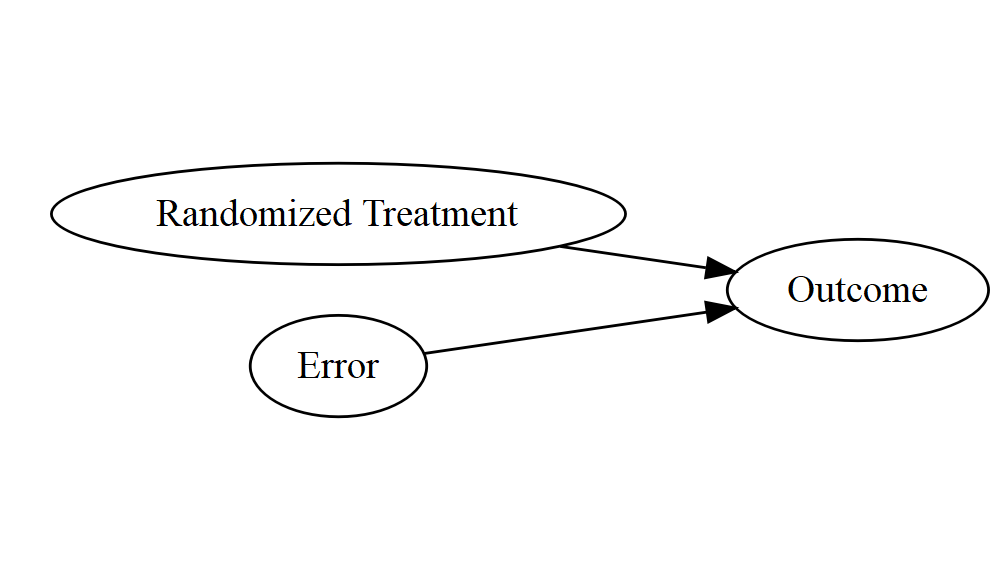
\includegraphics[width=\maxwidth]{figure/explanation1-1} 

\end{knitrout}
\end{frame}

\begin{frame}
\frametitle{Independent Treatment Assignment}
\begin{itemize}
\item But our logic works only based on \textbf{expectations} (averages)
\pause
\begin{itemize}
\item \textit{On average}, potential outcomes will be balanced
\pause
\item That's more likely in larger samples
\pause
\item Less likely in small samples; by chance, potential outcomes may be biased
\pause
\item We have no way of \textit{verifying} if potential outcomes are biased
\end{itemize}
\end{itemize}
\end{frame}

\section{Analyzing Field Experiments}

\begin{frame}
\frametitle{Analyzing Field Experiments}
\begin{itemize}
\item If treatment is random we know that:
$$E(Y_1|D=1) - E(Y_0|D=0) = E(Y_1) - E(Y_0) $$
\pause
\item What is $E(Y_1|D=1)$? 
\pause 
\item What is $E(Y_0|D=0)$?
\pause
\item This is easy! 
\pause
\item Just the difference in outcome means between treatment and control units
\pause
\begin{itemize}
\item And a simple T-test for statistical significance
\pause
\item NO modelling assumptions (``non-parametric'')
\end{itemize}
\end{itemize}
\end{frame}

\begin{frame}
\frametitle{Analyzing Field Experiments}
\begin{itemize}
\item Simple Regression $=$ Difference-in-means T-test
\pause
$$Y_i \sim \alpha + \beta D_i = \epsilon_i$$
\pause
$$Y_i = Y_{0i} + (Y_{1i} - Y_{0i}) D_i + \epsilon_i$$
\pause
\end{itemize}
\end{frame}

\begin{frame}
\frametitle{Analyzing Field Experiments}
\begin{itemize}
\item Simple Regression $=$ Difference-in-means T-test
\pause
\footnotesize
\item T-test Results:
% latex table generated in R 3.5.2 by xtable 1.8-3 package
% Fri Mar 29 10:11:31 2019
\begin{table}[ht]
\centering
\begin{tabular}{rrrr}
  \hline
 & estimate & statistic & p.value \\ 
  \hline
1 & 0.27065 & 2.69475 & 0.00706 \\ 
   \hline
\end{tabular}
\end{table}

\pause
\item Regression Results:
% latex table generated in R 3.5.2 by xtable 1.8-3 package
% Fri Mar 29 10:11:31 2019
\begin{table}[ht]
\centering
\begin{tabular}{rlrrrr}
  \hline
 & term & estimate & std.error & statistic & p.value \\ 
  \hline
1 & (Intercept) & 0.03459 & 0.07110 & 0.48647 & 0.62664 \\ 
  2 & treatment & 0.27065 & 0.10044 & 2.69472 & 0.00706 \\ 
   \hline
\end{tabular}
\end{table}

\end{itemize}
\normalsize
\end{frame}

\begin{frame}
\frametitle{Analyzing Field Experiments}
\begin{itemize}
\item How do we randomize?
\begin{itemize}
\item Hard! We can't just 'pick' treated units off the top of our heads
\pause
\item Computers are deterministic
\pause
\item The best we can do is to use atmospheric noise or radioactive decay
\pause
\end{itemize}
\item In the real world, randomization is hard
\begin{itemize}
\item Pressure to help the most needy
\pause
\item Political pressure
\pause
\item We don't want to be guinea pigs!
\end{itemize}
\end{itemize}
\end{frame}

\begin{frame}
\frametitle{Analyzing Field Experiments}
\begin{itemize}
\item How do we randomize?
\pause
\item So how do we confirm that randomization has succeeded?
\pause
\begin{itemize}
\item We can't directly test potential outcomes
\end{itemize}
\begin{enumerate}
\item \textbf{Qualitative research:} to reconstruct the treatment process
\pause
\item \textbf{Balance tests:} We can directly test other variables between treatment and control
\begin{itemize}
\item Randomization balances \textit{all} variables, not just potential outcomes
\end{itemize}
\end{enumerate}
\end{itemize}
\end{frame}


\section{Implementing Field Experiments}

\section{Designing Field Experiments}

\end{document}

%Random sample vs. Random treatment
%why 50:50

%\pause
%\item But we can assess balance in \textit{observable} covariates
%\item What if some covariates are imbalanced? %Expected 1/20. Still need to correct as could be real bias.


%setwd('C:\\Users\\Jonny\\Google Drive\\Academic\\USP\\Class\\Week 1 - Intro\\Lecture Slides')
%knitr::knit("Slides_Wk1_intro_5.Rnw")
